\documentclass[11pt]{article}
\usepackage[left=2cm, right=2cm, top=2cm, bottom=2cm]{geometry}
\pagenumbering{arabic}
\usepackage{footnote}
\usepackage{graphicx}
\usepackage{amsmath}
\usepackage[font={footnotesize}]{caption}
\usepackage{natbib}
\usepackage{wrapfig}
\usepackage{color}
\usepackage{setspace}
\usepackage{url}
\usepackage{fancyhdr}
\usepackage{enumitem}
\usepackage{hyperref}

\hypersetup{
    colorlinks=true,
    linkcolor=black,
    filecolor=magenta,      
    urlcolor=blue,
    citecolor=black
}

\setlength{\bibsep}{1pt}

\pagestyle{fancyplain}
\lfoot{\small Rebecca Smethurst}
\rfoot{\small Research Proposal}
\lhead{}
\rhead{}

\renewcommand{\headrulewidth}{0pt}
\renewcommand{\refname}{\normalfont\selectfont\normalsize\bf References}

\def\lesssim{\mathrel{\hbox{\rlap{\hbox{\lower3pt\hbox{$\sim$}}}\hbox{\raise2pt\hbox{$<$}}}}}

\definecolor{nc}{rgb}{0,0,0}
\def\changed{\color{nc}}

\title{{\bf \large \vspace{-2.5em} Searching for observational evidence of AGN feedback}\vspace{-1.0em}}
\author{\normalsize \vspace{-1.5em} Rebecca Jane Smethurst - Research Proposal}
\date{}

\begin{document}
\maketitle

%%%%%%%%%%%%%%%%%%%%%%%%%%%% PLAN %%%%%%%%%%%%%%%%%%%%%%%%%%%%
%
% INTRO: Galaxy Evo, previously reduced to single numbers, importance of understanding why SF stopes, complex systems
% PARA 1: GZ awesome + SDSS - breakthroughs in understanding of morphology over large populations
% PARA 2: BLACK HOLES - also thought to impact SD, morphology, ultimate drivers internally - external different
% PARA 3: Bayesian stats evidence + GZ + SPS = BH hosts undergone quenching recently, rapidly across whole population - but CAUSE or CONSEQUENCE? INTERNAL OR EXTERNAL?
% PLOT 1: medium mass agn time and rate
% PARA 4: MaNGA saves the day - IFUs - 127 fibers, 10000 galaxies - spatially reduced spectra - Li et al prelim - want to do using Bayesian sats and large populations
% PARA 5: HI data also crucial - gas fraction gives more info - observing proposal GBT to ensure entire MaNGA sample covered - lead Karen - who will work with 
% PARA 6: Portsmouth is perfect place - 1 of 2 places in UK with full buy in - lead data scientist - SPS experts
%%%%%%%%%%%%%%%%%%%%%%%%%%%%%%%%%%%%%%%%%%%%%%%%%%%%%%%%%%%%%%

Since the first discovery of galaxies in our Universe, understanding their evolution has progressed via analyses that reduce a galaxy into a single aperture. That era is now at an end. The current barrier to our comprehension of galaxy evolution is understanding the complex mechanisms controlling the shutdown (or `quenching') of star formation. In my previous work I have focused on this problem by applying a novel Bayesian inference code \citep[first described in][]{smethurst15} to analyse the star formation histories (SFHs) of galaxies. I propose to build significantly on this work by utilising data from the MaNGA (Mapping Nearby Galaxies at Apache Point Observatory; \citealt{Bundy15}) survey, which will provide a spectrum at 127 individual points (`spaxels') in each of the 10,000 galaxies targeted, making it the largest of its kind (see maps of resolved spectral features in Figure~\ref{gal}). If awarded this Junior Research Fellowship, I propose to use my novel inference code to determine whether quenching due to feedback from active galactic nuclei (AGN) occurs across the observable galaxy population? 

\vspace{-0.5em}

\begin{figure}[h]
\begin{centering}
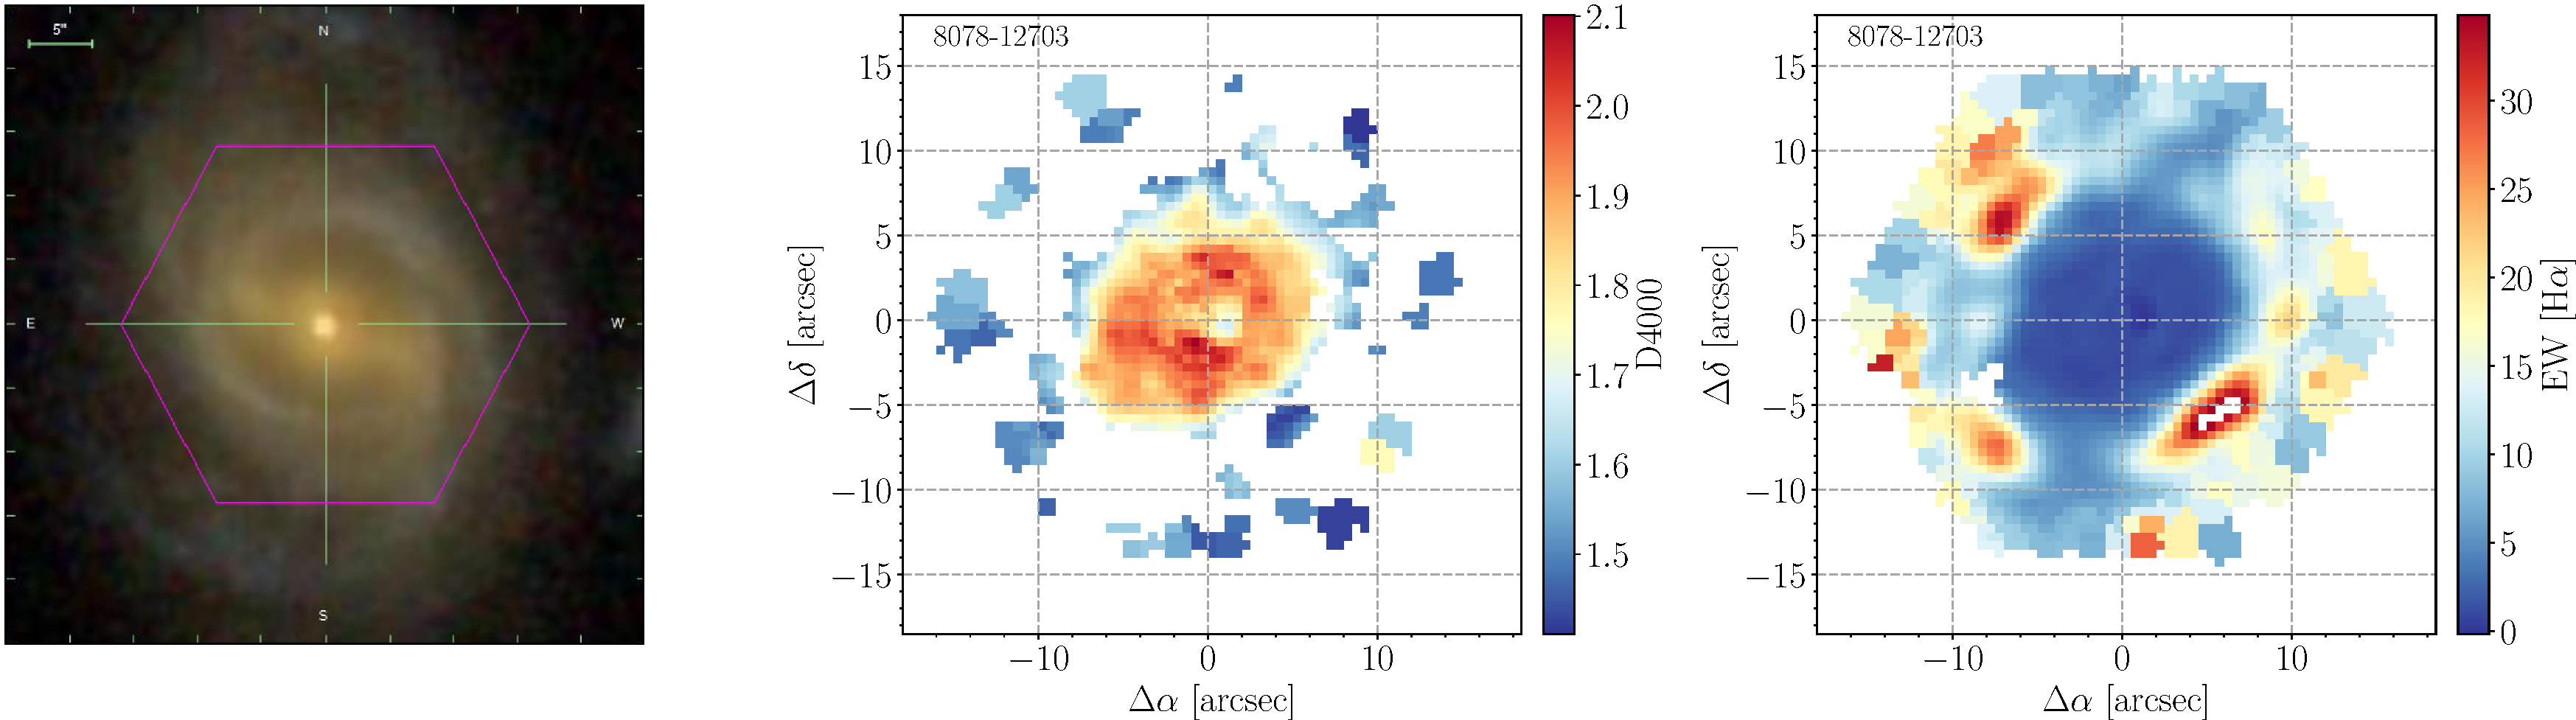
\includegraphics[width=0.8\textwidth]{image_halpha_vel_map_8078-12703_gal_aligned_ifu_bundles-MAPS-VOR10-GAU-MILESHC.pdf}
\vspace{-0.5em}
\caption[8pt]{Image of an example galaxy observed by MaNGA (left) showing the spectral fibre coverage (magenta) with corresponding data showing the spectral index D4000 (middle, a tracer of stellar age) and equivalent width of the $H\alpha$ emission line (right, a tracer of star formation) resolved across the galaxy in each of the spaxels.}
\label{gal}
\end{centering}
\vspace{-1.5em}
\end{figure}
\vspace{-0.5em}

\section*{\large Motivation}
\vspace{-0.5em}

\indent An AGN is a growing supermassive black hole (SMBH) in the centre of a galaxy. %There are tight correlations between properties of galaxies and central black hole mass, suggesting that changes in galaxy properties, such as star formation rate (SFR), could also be tied to the black hole activity. 
AGN feedback is thought to occur via the output of energetic material and radiation from accretion onto a SMBH. This output is  assumed to either heat or expel hydrogen gas from a galaxy, removing critical fuel for future star formation. There are strong theoretical predictions for AGN feedback occurring across the entire galaxy population \citep{Fabian12, Gaibler12}. For example, without AGN feedback to regulate star formation, simulated galaxies grow to unrealistic stellar masses \citep[e.g.][]{silk12}. However, direct observational evidence for quenching caused by AGN across the galaxy population has been elusive. This persistent lack of proof for AGN feedback continues to challenge our basic understanding of how the Universe evolves. 

However, by employing my novel inference code\footnote{\url{https://github.com/zooniverse/starpy}} I have been able to show that a population of nearby AGN host galaxies have undergone a recent, rapid decline in star formation, not detected in a control sample of galaxies with inactive SMBHs (see peaks at recent times and rapid rates in Figure \ref{timerate}). This finding of recent, rapid quenching suggests that AGN feedback is the cause, as AGN have short lifetimes of $\lesssim0.3$~Gyr \citep{martini04} and in simulations are found to cause rapid quenching \citep{tortora09}. %This is a profound result, inferred using only two galaxy colours. 
However, using this data I am not able to determine whether AGN feedback is the internal cause of the inferred quenching or whether the AGN is merely a consequence of another external quenching mechanism (e.g. its activity has been triggered by a galaxy interaction or merger). 

\begin{figure}[t]
\begin{centering}
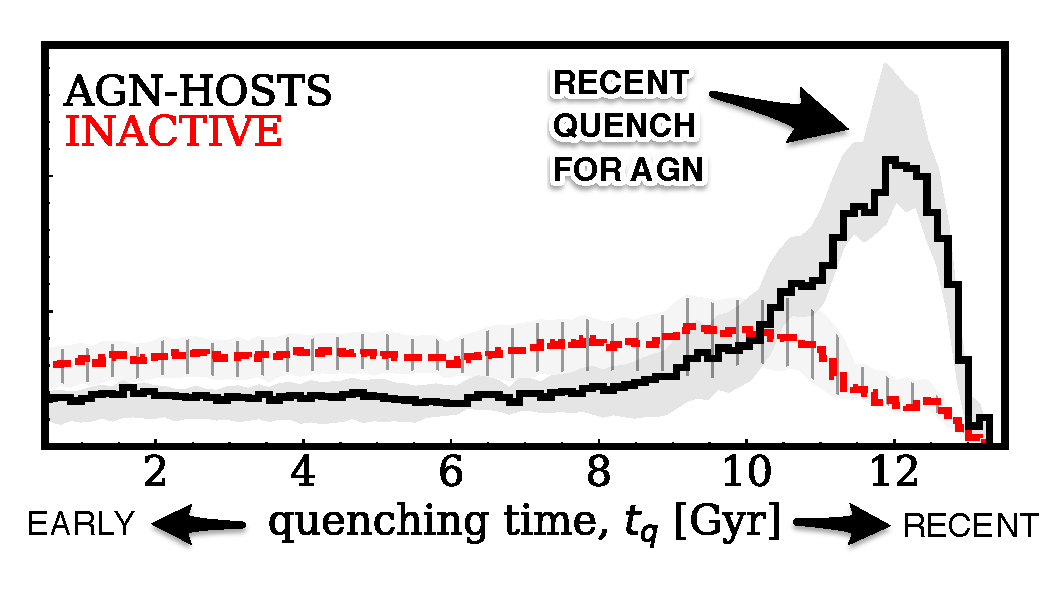
\includegraphics[width=0.375\textwidth]{quenching_time_all_masses_bootstrap_one_morphology.pdf}
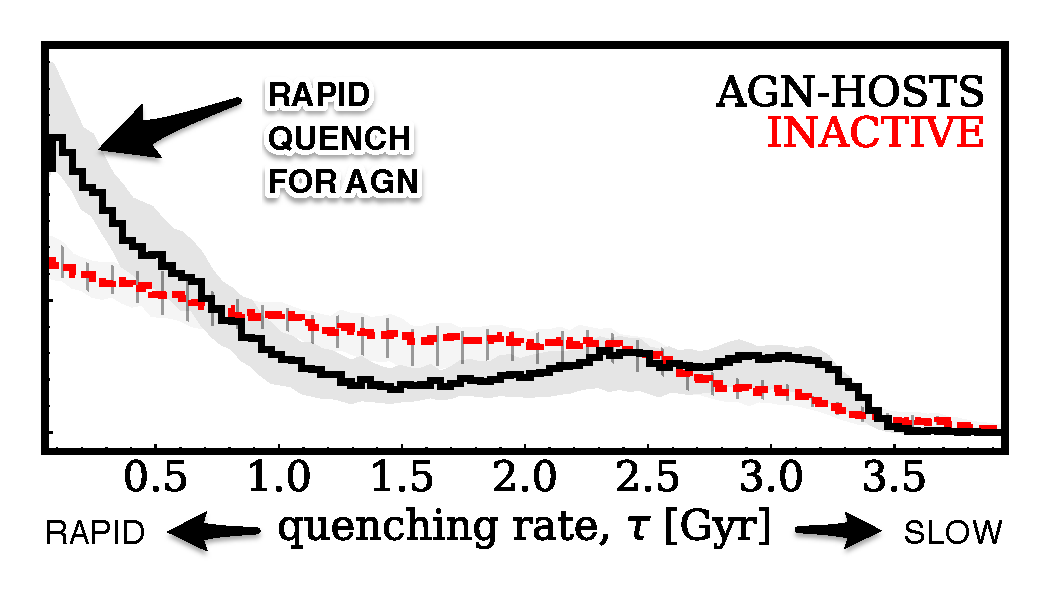
\includegraphics[width=0.375\textwidth]{quenching_rate_all_masses_bootstrap_one_morphology.pdf}
\vspace{-0.5em}
\caption[8pt]{The difference in the time (left) and rate (right) of quenching in nearby galaxies that host AGN (black, solid) compared to galaxies with inactive SMBHs (red, dashed). The plots are normalised so that the areas underneath the curves are equal. The peaks in the black, solid lines show that recent ($\sim12~\rm{Gyr}$ left panel), rapid ($\sim0.1~\rm{Gyr}$ right panel) quenching is occurring in the AGN host galaxy population, which is not seen in the inactive galaxy population (red dashed lines), suggesting this quenching may be caused by AGN feedback. Adapted from Figures $4$ \& $5$ in \cite{smethurst16}.}
\label{timerate}
\end{centering}
\vspace{-1.5em}
\end{figure}

\vspace{-0.5em}
\section*{\large Proposed research}
\vspace{-0.5em}

I propose to use data from the MaNGA survey to infer spatially resolved SFHs of galaxies. I will adapt my code to use star formation, age and metallicity sensitive spectral parameters %(see spatially resolved age and star formation sensitive spectral features in Figure~\ref{gal}), 
to infer more precise SFHs than derived previously from galaxy colours. I propose to use these spatially resolved SFHs to answer the following science questions:

\begin{enumerate}[leftmargin=*]

\item {\bf Are AGN causing quenching through feedback?} I will investigate whether the spatially resolved SFHs of AGN host galaxies are statistically distinguishable from those hosting inactive SMBHs. In particular I will determine if the expected signatures of AGN feedback are present in the spatially resolved SFHs. If I find a statistical correlation between the distance from the central AGN and the time that quenching has occurred, this will provide direct evidence for AGN feedback via the radiation of energy outward through the galaxy.

\item {\bf Does a galaxy's SFH correlate with properties of the SMBH?} There are tight correlations between the bulge \& total stellar mass of a galaxy, and SMBH mass \citep{haring04}, implying a co-evolution. Mergers have long been considered the dominant mechanism for this simultaneous growth of SMBHs and galaxies, and are thought to power the most energetic AGN \citep{hopkins08, treister12}. However, recent results from \citet[]{simmons17} have shown that galaxies with merger-free histories host SMBHs 100 times more massive than expected, suggesting that secular mechanisms play a greater role in feeding SMBHs. I propose to investigate which mechanisms are triggering AGN feedback by determining if there are statistical differences between the spatially resolved SFHs of AGN host galaxies which have and have not undergone a merger. This will allow me to determine whether AGN feedback is important for the entire galaxy population or whether it only dominates in a certain region of parameter space. 

\end{enumerate}

I have been working with MaNGA data during my current fellowship at the University of Nottingham and so I am already experienced in handling the data and its corresponding analysis tools. This puts me in a unique position to successfully complete this proposed research with my combined knowledge of the data, the statistical techniques and my inference code. This research will provide both an analysis tool for the astrophysical community and a statistical test of a long standing 	problem, allowing us to better inform our understanding of the Universe.
% \vspace{-0.5em}

% \section*{\large Summary}
% \vspace{-0.5em}

% If awarded this fellowship, I will apply my adapted SFH inference code to MaNGA data to test whether quenching caused by AGN feedback occurs across the galaxy population. I expect to publish at least three papers documenting this research; the first describing my adapted inference code (2018-2019), the second detailing evidence, or otherwise, for AGN feedback across a star formation independent sample of AGN hosts (2019-2020) and a third determining where AGN feedback is a dominant mechanism (2020-2021). 


\vspace{-0.5em}

\begin{thebibliography}{}
{\fontsize{7.5pt}{2pt}\selectfont
\begin{minipage}[t]{0.3\textwidth}
\bibitem[\protect\citeauthoryear{Bundy et al.}{2015}]{Bundy15} Bundy, K. et al. 2015, ApJ, 798, 7
\bibitem[\protect\citeauthoryear{Fabian}{2012}]{Fabian12} Fabian, A. C. 2012, ARA\&A, 50, 455
\bibitem[\protect\citeauthoryear{Gaibler et al.}{2012}]{Gaibler12} Gaibler, V. et al. 2012, MNRAS, 425, 438
\bibitem[\protect\citeauthoryear{H\"aring \& Rix}{2004}]{haring04} H\"aring N. \& Rix H.-W. 2004, ApJ, 604, L89
\bibitem[\protect\citeauthoryear{Hopkins et al.}{2008}]{hopkins08} Hopkins P. et al. 2008, ApJS, 175, 356 
\end{minipage}
\hspace{0.5cm}
\begin{minipage}[t]{0.3\textwidth}
\bibitem[\protect\citeauthoryear{Martini}{2004}]{martini04} Martini, P., 2004, Coevolution of Black Holes and Galaxies, 169

\bibitem[\protect\citeauthoryear{Silk \& Mamon}{2012}]{silk12} Silk J., Mamon G. A., 2012, Research in Astronomy and Astrophysics, 12, 917
\bibitem[\protect\citeauthoryear{Simmons, Smethurst \& Lintott}{2017}]{simmons17} Simmons, B. D. ; Smethurst, R. J. \& Lintott, C. J. 2017, MNRAS, 470, 1559 
\end{minipage}
\hspace{0.5cm}
\begin{minipage}[t]{0.3\textwidth}
\bibitem[\protect\citeauthoryear{Smethurst et al.}{2015}]{smethurst15} Smethurst, R. J. et al. 2015, MNRAS, 450, 435
\bibitem[\protect\citeauthoryear{Smethurst et al.}{2016}]{smethurst16} Smethurst, R. J. et al. 2016, MNRAS, 463, 2986
%\bibitem[\protect\citeauthoryear{Smethurst et al.}{2017}]{smethurst17a} Smethurst, R. J. et al. 2017, MNRAS, 469, 3670
% \bibitem[\protect\citeauthoryear{Smethurst et al.}{2017b}]{smethurst17b} Smethurst, R. J. et al. 2017b, MNRAS, \emph{stx2547}
%\bibitem[\protect\citeauthoryear{Springel, Di~Matteo \& Hernquist}{2005}]{Springel05} Springel, V., Di Matteo, T. \& Hernquist, L., 2005, ApJ, 620, L79
\bibitem[\protect\citeauthoryear{Tortora et al.}{2009}]{tortora09} Tortora C. et al. 2009, MNRAS, 396, 61
\bibitem[\protect\citeauthoryear{Treister et al.}{2012}]{treister12} Treister E. et al. 2012, ApJ, 758, L39
\bibitem[\protect\citeauthoryear{Urry \& Padovani}{1995}]{urry95} Urry C. M., Padovani P., 1995, PASP, 107, 803

\end{minipage}
\par}
\end{thebibliography}

\end{document}